In this chapter planning and work-flow regarding Sprint 3 will be described. 
All from setting our goals to implementation and testing. On the end we will evaluate whole sprint and try to answer on following questions: What went well? What could be improved? What should we start doing?  
% TODO rewrite

\section{Sprint planning}
% TODO

This time we offered customer to have a "pre-demo" video on Thursday 4.10.2013 during our regular meeting.
\subsection{Duration}
This sprint will be 2 weeks long. From 30.09.2013 to 13.10.2013.
We agreed on the date of presentation and showing the running demo - Thursday 11.10.2013.
Estimated velocity is 240h since we agreed on 30 working hours per person per week.

\subsection{User-stories}
You can see user stories concerning sprint 3 in table \ref{tab:sprint3stories}.
\LTXtable{\textwidth}{sprint3/stories.tex}
\subsection{Sprint goal}
The goal of this sprint is having a working application on a mobile phone that can work in two modes.  
Input type and output are for both modes common - input is an image or video and output is location of detected mobile phones in a given matrix (e.g. 4x4 matrix) with color that mobile's screen is lighting.
In the first mode, real video from mobile's camera will be treated as an input and on the other hand in the second mode mock data (image/video) are treated as an input.

You can see example of input with matrix 2x2 in image. Appropriate output of image processing and mapping module will be: \texttt{\{blue,[0,0]\}, \{red,[0,1]\}, \{green,[1,1]\}}.

\begin{figure}[H]
	\centering
		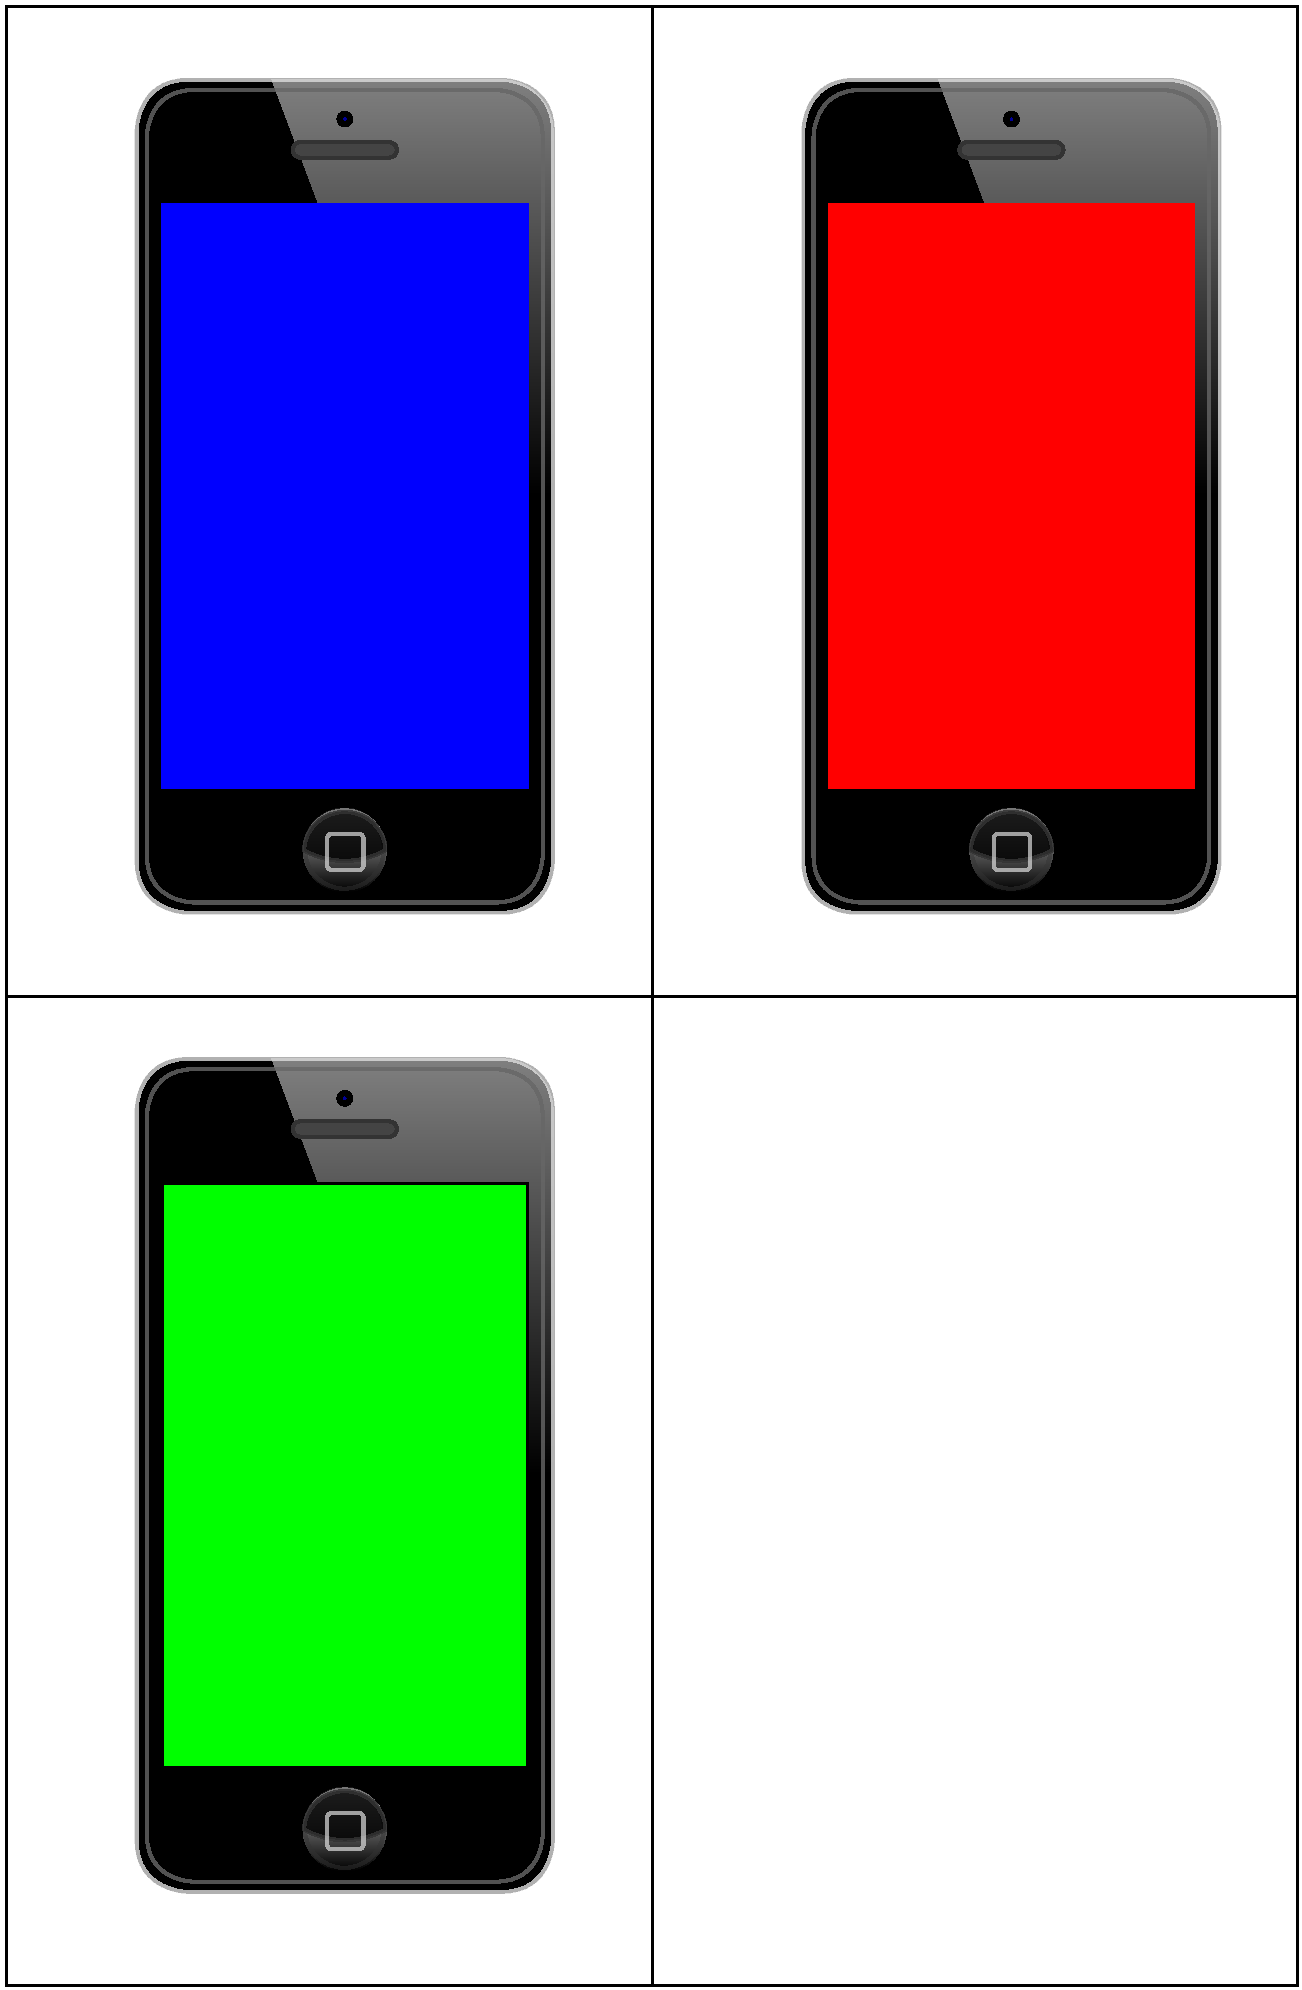
\includegraphics[width=7cm]{sprint3/sprint3_goal.pdf}
	\caption{Example of ideal data input for image processing module with 2x2 matrix.}
	\label{img:sprint3_goal}
\end{figure}

\section{System Burndown}
\section{Architecture}
\section{Implementation}
\section{Testing}
\section{Occurring risks}
\section{Retrospective}
\subsection{Pros}
\subsection{Cons}
\section{Evaluation}